\documentclass[12pt,compress]{beamer}
%\documentclass[handout,t]{beamer}

\batchmode
% \usepackage{pgfpages}
% \pgfpagesuselayout{4 on 1}[letterpaper,landscape,border shrink=5mm]

\usepackage{amsmath,amssymb,enumerate,epsfig,bbm,calc,color,ifthen,capt-of,multicol,wrapfig,cutwin}

\usepackage[all,pdf]{xy}

% add page number
\expandafter\def\expandafter\insertshorttitle\expandafter{%
	\insertshorttitle\hfill%
	\insertframenumber\,/\,\inserttotalframenumber}

\usetheme{Berlin}
\usecolortheme{umji}

\title{Chemical Thermodynamics}
\subtitle{Mid 2 Review}
\author{Haotian Fu}
\institute{University of Michigan--Shanghai Jiao Tong University Joint Institute}
\date{\today}

\AtBeginSection[]
{
  \begin{frame}<beamer>
    \frametitle{Outline}
    \tableofcontents[currentsection]
  \end{frame}
}
\beamerdefaultoverlayspecification{<+->}

% -----------------------------------------------------------------------------
\begin{document}

% -----------------------------------------------------------------------------

\lecture{RC_3}

\frame{\titlepage}

\section[Outline]{}
\begin{frame}{Outline}
    \tableofcontents
\end{frame}

% -----------------------------------------------------------------------------

\section{Concept Review}
\subsection{Thermodynamic Laws}
\begin{frame}{Thermodynamic Laws}
    \begin{block}{1$^{\text{st}}$ Law}
        U = Q + W
    \end{block}
    \begin{block}{2$^{\text{nd}}$ Law}
        100 \% ($\times$)
    \end{block}
    \begin{block}{3$^{\text{rd}}$ Law}
        S $\rightarrow$ c as T $\rightarrow$ 0 K \\
        S = kln W
    \end{block}
\end{frame}
\begin{frame}{Do not forget the zeroth law of thermodynamics}
    \begin{block}{0$^\text{th}$ Law}
        If two thermodynamic systems are each in thermal equilibrium with a third system, then they are in thermal equilibrium with each other.
    \end{block}
\end{frame}
\begin{frame}{State functions}
    \begin{block}{Enthalpy}
        H = U + pV
    \end{block}
    \begin{block}{Entropy}
        dS = $\frac{\delta \text{Q}}{\text{T}}$
    \end{block}
    \begin{block}{Gibb's free energy}
        G = H - TS
    \end{block}
\end{frame}
\begin{frame}{Properties}
    \begin{block}{Heat capacity}
        C = $\lim\limits_{\Delta \text{T} \rightarrow 0}\frac{\Delta \text{Q}}{\Delta \text{T}}$
    \end{block}
    \begin{figure}[H]
        \centering
        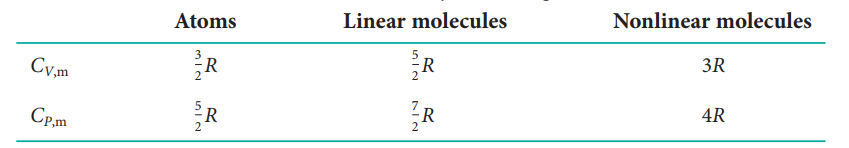
\includegraphics[width=\textwidth]{KMT.png}
        \caption{$C_{V,m}$ and $C_{p,m}$ of three types of molecules.}
    \end{figure}
\end{frame}

\subsection{Practical Formula}
\begin{frame}{Practical Formula}
    \begin{align}
         & Q_V = \Delta U                                      \\
         & Q_p = \Delta H                                      \\
         & C_V = \frac{\Delta U}{\Delta T}                     \\
         & C_p = \frac{\Delta H}{\Delta T}                     \\
         & \Delta S_{\text{surrounding}} = -\frac{\Delta H}{T} \\
         & S=k\ln W
    \end{align}
\end{frame}
\begin{frame}{Practical Formula}
    \begin{align}
         & \text{phase change } \nonumber                                                         \\
         & \Delta S = \frac{Q_R}{T}                                                               \\
         & \text{physical change with constant pressure } \nonumber                               \\
         & \Delta S = nC_{V,m}\ln\left(\frac{T_2}{T_1}\right) + nR\ln\left(\frac{V_2}{V_1}\right) \\
         & \text{physical change with constant volume } \nonumber                                 \\
         & \Delta S = nC_{p,m}\ln\left(\frac{T_2}{T_1}\right) + nR\ln\left(\frac{p_1}{p_2}\right)
    \end{align}
\end{frame}
\begin{frame}{Practical Formula}
    \begin{align}
         & \text{Clausius–Clapeyron relation} \nonumber                                                  \\
         & \ln\left(\frac{p_2}{p_1}\right) = -\frac{\Delta H}{R}\left(\frac{1}{T_2}-\frac{1}{T_1}\right) \\
         & \text{constant temperature} \nonumber                                                         \\
         & \Delta G = \int V dp \quad \text{since}\quad dG = -sdT + Vdp
    \end{align}
\end{frame}

% -----------------------------------------------------------------------------

\section{Classic Models}

\subsection{Free expansion}
\begin{frame}{Free expansion}
    \begin{block}{Differential form}
        $\delta$ w = -pdV
    \end{block}
    \begin{block}{Notice}
        \begin{itemize}
            \item $\Delta U$ = 0 and $\Delta H$ = 0 for isothermal processes.
            \item w = 0 for free expansion.
            \item p is external pressure, \textit{i.e.}, p = p$_\text{ex}$.
        \end{itemize}
    \end{block}
\end{frame}

\subsection{Calimeter}
\begin{frame}{Calimeter}
    \begin{figure}
        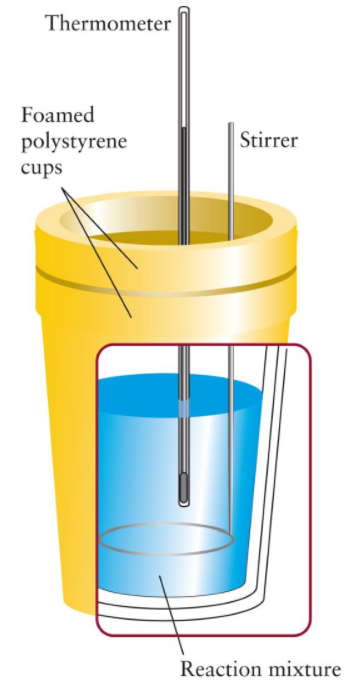
\includegraphics[height=0.8\textheight]{Calimeter.png}
    \end{figure}
\end{frame}
\begin{frame}{Calimeter}
    \begin{block}{Notice}
        \begin{itemize}
            \item Combustion reaction.
            \item Q = Q$_\text{V}$ $\Rightarrow$ $\Delta U$
            \item Specific heat of water: 4.18 J/(g $\cdot$ $^\circ$C)
        \end{itemize}
    \end{block}
\end{frame}

\subsection{Heating curve}
\begin{frame}{Heating curve \& Phase diagram}
    \begin{block}{Notice}
        \begin{itemize}
            \item Phase changes of materials.
            \item Turning points.
            \item Intervals, platforms, and slopes.
        \end{itemize}
    \end{block}
\end{frame}

\subsection{Trouton’s rule}
\begin{frame}{Trouton's rule}
    \begin{figure}[H]
        \centering
        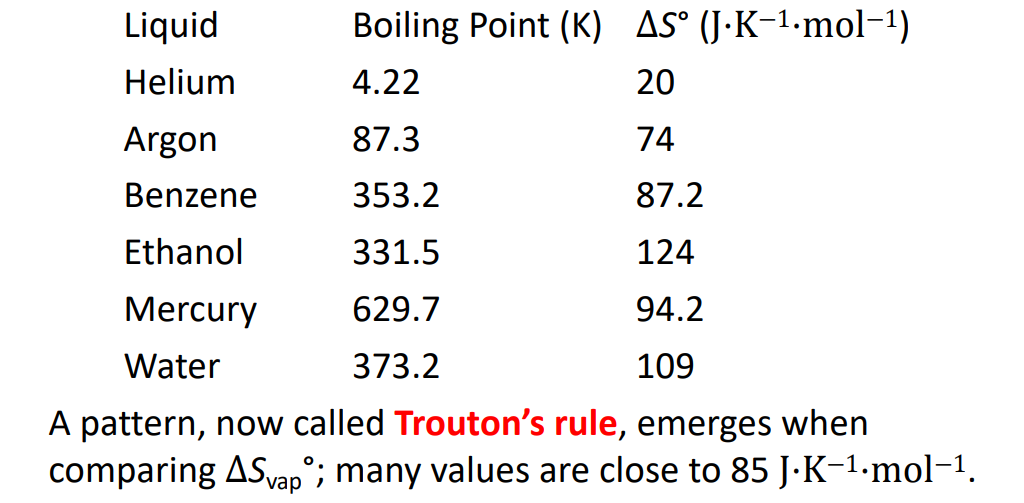
\includegraphics[width=\textwidth]{Trouton.png}
    \end{figure}
    \begin{itemize}
        \item Semi-quantitative, not precise.
    \end{itemize}
\end{frame}

\subsection{State function}
\begin{frame}{State function}
    \begin{itemize}
        \item Pay attention to initial and final state.
        \item Pay attention to dependent variables.
        \item \textcolor{red}{Design desired cycles.}
    \end{itemize}
\end{frame}
\begin{frame}{How to design a cycle?}
    \begin{block}{Thermodynamic processes}
        \begin{itemize}
            \item Constant conditions: isothermal, isochoric, isobaric, (adiabatic)
            \item Energy dissipation: reversible, irreversible
        \end{itemize}
    \end{block}
    \begin{block}{Properties of state functions}
        \begin{itemize}
            \item Only related to initial and final state, \textcolor{red}{nothing to do with paths}.
            \item From already known to unknowns, set proper path and intermediate state.
        \end{itemize}
    \end{block}
\end{frame}

\subsection{Examples}
\begin{frame}{Lecture slides}
    \begin{figure}[H]
        \centering
        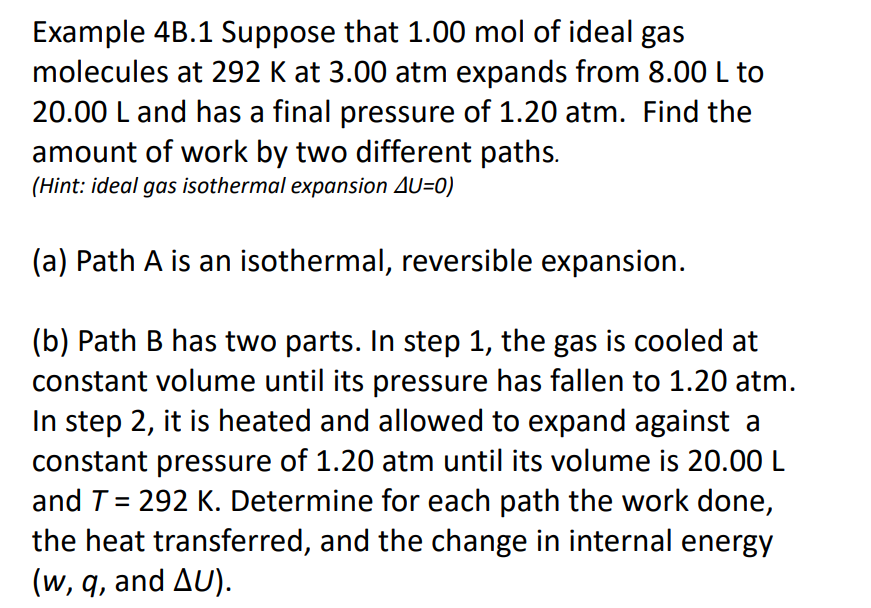
\includegraphics[height=0.8\textheight]{example.png}
    \end{figure}
\end{frame}
\begin{frame}{Lecture slides}
    \begin{figure}[H]
        \centering
        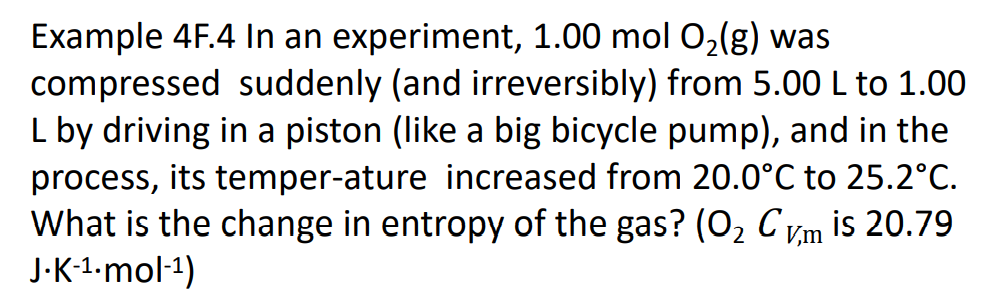
\includegraphics[width=\textwidth]{slides.png}
    \end{figure}
\end{frame}
\begin{frame}{Lecture slides}
    \begin{figure}[H]
        \centering
        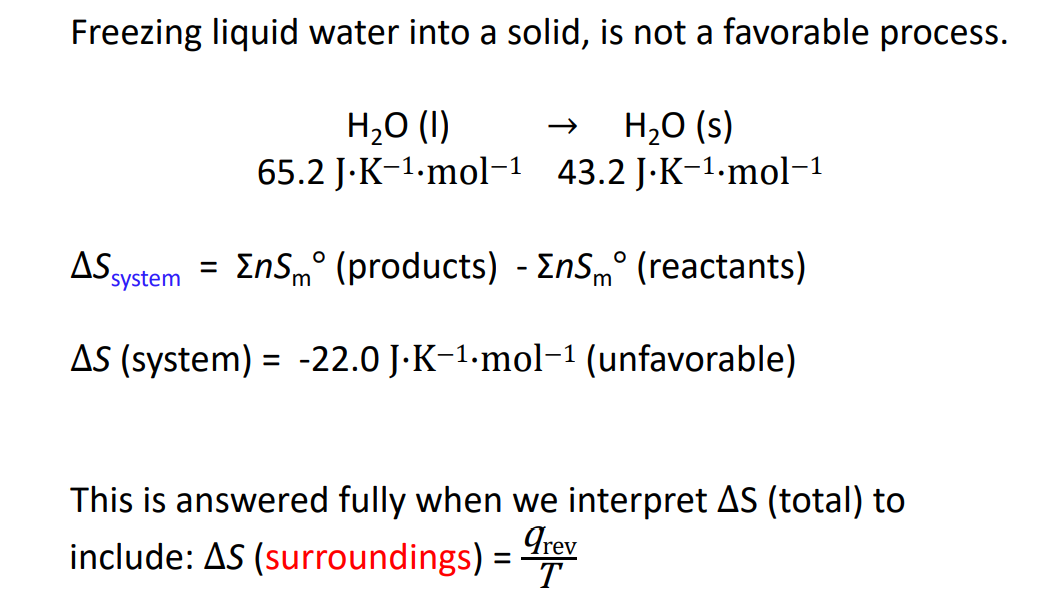
\includegraphics[width=\textwidth]{rev_phase.png}
    \end{figure}
\end{frame}
\begin{frame}{Lecture slides}
    \begin{figure}[H]
        \centering
        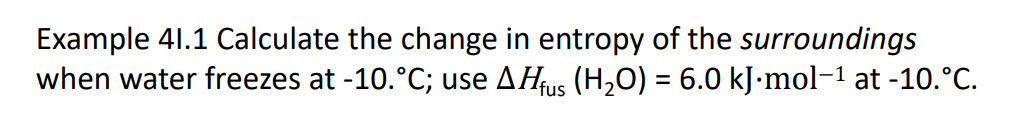
\includegraphics[width=\textwidth]{S_sur.png}
    \end{figure}
\end{frame}



\begin{frame}{Bohn-Haber Cycle}
    \begin{block}{Design desired cycle}
        The standard molar enthalpy of combustion of ethanol (C$_2$H$_5$OH) and acetic acid (CH$_3$COOH) is -136.50 and -67.50 kJ/mol. \\
        The enthalpy of dissolution is 11.71 and 1.46 kJ/mol correspondingly. Calculate the enthalpy of oxidation of thtanol in water solution.
    \end{block}
\end{frame}
\begin{frame}{Liquid-Solution}
    \begin{block}{Raoult's law and Dalton's law}
        Liquid $A$ and $B$ form an ideal solution. The solution containing 1 mol $A$ and 2 mol $B$ at 343.2 K has a vapor pressure of 50.663 kPa. \\
        If 3 mol $A$ is added, the vapor pressure of the solution increases to 70.928 kPa. Calculate (1) $p_A^*$ and $p_B^*$ at 343.2 K; (2) the gaseous composition of the first mixed solution.
    \end{block}
\end{frame}

%------------------------------------------------------------------------------

\begin{frame}{}
    \textbf{{\Huge{Good Luck !}}}
\end{frame}

\end{document}